\documentclass{article}
\usepackage[T1]{fontenc}
\usepackage[utf8]{inputenc}
\usepackage{lmodern}
\usepackage{textcomp}
\usepackage{lastpage}
\usepackage{tikz}
\usepackage{amsmath}
\usepackage{graphicx}
\usepackage{float}
%\setcounter{secnumdepth}{0}

\title{Mathématiques Financières}
\author{Licence 3}
\date{2021 - 2022}

\begin{document}
\normalsize
\maketitle

\renewcommand*\contentsname{Table des matières}
\tableofcontents
\newpage

\section{Introduction}
Ce cours traite la valeur acquise par un capital, avec soit :


\begin{itemize}
   \item un versement initial unique,
   \item des versements constants à chaque période.
\end{itemize}

\section{Résumé des formules}

{
\large
$$ V_n = C\cdot(i+1)^n$$

$$i_m = (i+1)^{\frac{1}{12}} - 1$$

$$V_{act} = \dfrac{V_f}{(\tau+1)^n}$$

$$V^{deb}_{acq} = a(i+1)\cdot\dfrac{(i+1)^n-1}{i}$$

$$V^{deb}_{act} = a(\tau+1)\cdot\dfrac{1-\frac{1}{(\tau+1)^n}}{\tau}$$
}




\newpage
\section{Versement initial unique}

\subsection{Capitalisation}
On investit un capital de départ et on cherche à savoir combien on gagnera plus tard : c'est la \textbf{capitalisation}. 
\\ On raisonne par unité de temps : les  \textbf{périodes} \textit{(une année en général)}.

\subsubsection{Au bout de 1 période}

\begin{figure}[h]
    \centering
    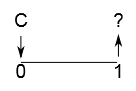
\includegraphics{c0-c1.png}
    \\On cherche la valeur à droite
\end{figure}

$$V = C\cdot(i+1)$$
avec :

- $C :$ capital de départ à la date 0

- $V :$ capital après $1$ période de temps

- $i :$ taux d'intérêt

\subsubsection{Au bout de $n$ périodes}

\begin{figure}[h]
    \centering
    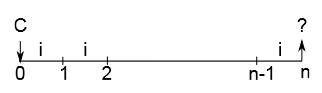
\includegraphics{c0-cn.png}
    \\On cherche la valeur à droite
\end{figure}

$$\boxed{V_n = C\cdot(i+1)^n}$$
avec :

- $C$ : capital initial

- $V_n$ : valeur capitalisée finale du placement


\subsection{Passage période annuelle à période mensuelle}
Soit $i$ le taux d'intérêt \textbf{annuel} et $i_m$ le taux d'intérêt \textbf{mensuel}.

\begin{figure}[H]
    \centering
    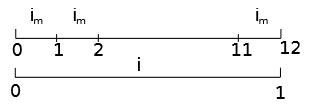
\includegraphics{i-im.png}
    \\On cherche $i_m$ à partir de $i$
\end{figure}

$$C(i_m+1)^{12} = C(i+1)$$ $$\implies \boxed{i_m = (i+1)^{\frac{1}{12}} - 1}$$


\subsection{Actualisation}
On veut savoir combien investir pour obtenir plus tard un capital défini : c'est l'\textbf{actualisation}.


\begin{figure}[h]
    \centering
    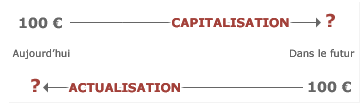
\includegraphics{capi-vs-actu.png}
    \\Capitalisation et actualisation
\end{figure}

\subsubsection{Au bout de 1 période}
$$V_{act} \times(\tau+1)= V_f$$

avec :

- $V_{act}$ : valeur actualisée (valeur aujourd'hui de $V_f$)

- $V_f$ : capital futur

- $\tau$ : taux d'actualisation

\subsubsection{Au bout de $n$ périodes}
$$V_{act} \times(\tau+1)^n= V_f$$
$$\implies \boxed{V_{act} = \dfrac{V_f}{(\tau+1)^n}}$$


\section{Versements constants}

\subsection{En début de période}
Ici, on ne suppose plus un versement initial, mais des versements constants en \textbf{début de période}, de valeur constante $a$.
\subsubsection{Capitalisation}

\begin{figure}[H]
    \centering
    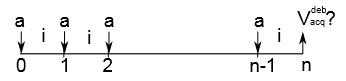
\includegraphics{versement-constant.png}
    \\On cherche la valeur à droite
\end{figure}

$$\boxed{V^{deb}_{acq} = a(i+1)\cdot\dfrac{(i+1)^n-1}{i}}$$

\subsubsection{Actualisation}

\begin{figure}[H]
    \centering
    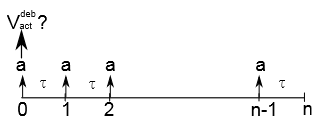
\includegraphics{versement-constant-actu.png}
    \\On cherche la valeur à gauche
\end{figure}

$$\boxed{V^{deb}_{act} = a(\tau+1)\cdot\dfrac{1-\frac{1}{(\tau+1)^n}}{\tau}}$$

\section {Jsp}
\subsection{VAN}
$$\boxed{VAN(\tau) = -V_0 + \sum_{i=1}^n \dfrac{V_i}{(1+\tau)^{p_i}}}$$
\subsection{TRI}
Le Taux de Rendement Interne $\tau_{tri}$ est une solution de l'équation 
$$VAN(\tau_{tri}) = 0$$
\end{document}
